%%% File encoding is UTF8

\chapter{Marco teórico}
\label{chp:marco_teorico}
Este capítulo tiene como objetivo entregar las bases teóricas, conceptuales y empíricas que soportan cada desarrollo de esta investigación. En primer lugar, se presenta el marco conceptual donde se entregan las definiciones y conceptos necesarios para abordar esta investigación. En segundo lugar, se presenta el estado del arte relacionado con el tema.


\section{Marco conceptual}
\label{sec:marco_conceptual}
En esta sección se presentan conceptos y bases teóricas respecto a la temática que conduce el desarrollo de este trabajo, el cual tiene relación con el uso de interfaces no tradicionales, específicamente con una interfaz operada con el cuerpo. Además, se indaga sobre ciertas definiciones para establecer lo que se pretende medir en este estudio, lo que involucra la experiencia de usuario y métricas de rendimiento en la realización de tareas. Finalmente, se proponen ciertas características fundamentales respecto de este tipo de proyectos relacionados con diseños experimentales con usuarios.

\subsection{Búsqueda de información}
\label{subsec:busqueda}

\subsection{Recuperación de Información Humano Computador}
\label{subsec:HCIR}
\ingles{Human Computer Information Retrieval} (HCIR) o Recuperación de Información Humano Computador\footnote{Traducción libre.}, es el estudio de los métodos que integran la inteligencia humana y la búsqueda algorítmica para ayudar a la gente a mejorar la búsqueda, exploración y aprendizaje de información (Marchionini, 2007). Dentro de esta área interactúan otras disciplinas, como la recuperación de información, llamada en inglés \ingles{Information Retrieval} (IR), la que está enfocada principalmente en proveer a los usuarios de fácil acceso a la información de su interés trabajando con la representación, almacenamiento, organización y acceso a objetos de información como documentos, páginas \ingles{web}, catálogos en línea y objetos multimedia (Baeza-Yates & Ribeiro-Neto, 2011) y la búsqueda de información, llamada en inglés \ingles{Information Seeking} (IS) que se entiende como un proceso más orientado al usuario y abierto que IR. En IS, no se sabe si existe una respuesta a la consulta del usuario, por lo que el proceso de búsqueda puede proporcionar el aprendizaje necesario para satisfacer su necesidad de información (Baeza-Yates & Ribeiro-Neto, 2011).

La búsqueda de información es un campo de la investigación que relaciona el desarrollo del área de las tecnologías y ciencias de la computación con la psicología y ciencias sociales en el procesamiento de la información, en donde el usuario toma un papel activo por medio de interacciones explicitas e implícitas con la información (Carroll, 1997).

Es una disciplina que contempla tanto al sistema como al usuario, así como la relación que se establece a través del comportamiento del usuario y sus experiencias (Kelly, 2009). Se ubica en un punto medio entre las disciplinas de HCI e IR.

\subsection{Rendimiento}
\label{subsec:rendimiento}
En el contexto de la recuperación de información se definen \ingles{precision} y \ingles{recall} en función de un conjunto de documentos relevantes y un conjunto de documentos recuperados (Powers, 2011), las cuales se definen a continuación.  

\begin{description}
	\item [\ingles{Precision}] Métrica que mide la razón de documentos relevantes recuperados con 
respecto al total de documentos recuperados. Es un valor continuo entre 0 y 1, mientras más cercano a 1, mayor fue su precisión al encontrar los documentos relevantes. La \eq{eq:precision} muestra
	\begin{equation}
	Precision = \frac{\big[\big\{documentos \ relevantes\big\} \cap \big\{documentos \ recuperados\big\}\big]}{\big\{documentos \ recuperados\big\}}
	\label{eq:precision}
	\end{equation}

	\item [\ingles{Recall}] Métrica que mide la razón de documentos relevantes recuperados con 
respecto al total de documentos relevantes. Es un valor continuo entre 0 y 1, mientras más cercano a 1, mayor fue la recuperación de documentos en base al total del universo disponible. La \eq{eq:recall} muestra
	\begin{equation}
	Recall = \frac{\big[\big\{documentos \ relevantes\big\} \cap \big\{documentos \ recuperados\big\}\big]}{\big\{documentos \ relevantes\big\}}
	\label{eq:recall}
	\end{equation}

	\item [\ingles{F1}] Métrica que considera a \ingles{precision} y \ingles{recall} en un promedio ponderado. Es un valor continuo entre 0 y 1, en que un valor cercano a uno permite identificar a los estudiantes con una recuperación de documentos proporcional a su precisión, respecto a la relevancia de estos. La \eq{eq:F1} muestra   
	\begin{equation}
	F1 = \frac{2 \cdot Precision\cdot Recall}{Precision+ Recall}
	\label{eq:F1}
	\end{equation}
 
	\item [\ingles{Coverage Effectiveness}] Razón entre la cobertura útil, páginas visitadas sobre 30 segundos, y el total de documentos visitados por un estudiante. Es un valor continuo entre 0 a 1, mientras más cercano a 1, mejor fue la efectividad de la cobertura respecto el universo de documentos, respecto al tiempo de permanencia. La \eq{eq:CE} muestra     
	\begin{equation}
	CE = \frac{UsfCover}{TotalCover}
	\label{eq:CE}
	\end{equation}

	\item [\ingles{Query Effectiveness}] Razón existente entre la efectividad de la cobertura (fórmula anterior) y el total de consultas realizadas por un estudiante. Esta proporción da indicios del desempeño del estudiante en torno a la calidad de las consultas efectuadas, en base a la cantidad y eficacia. Sus valores también están en un intervalo continuo entre 0 a 1. La \eq{eq:QE} muestra
	\begin{equation}
	QE = \frac{CE}{countQ}
	\label{eq:QE}
	\end{equation}

	\item [\ingles{Search Score}] Calificación de los estudiantes que se expresa en una escala continua de 0 a 5 puntos. Es una razón entre la cobertura relevante y el total de páginas marcadas activas al final de la tarea. La \eq{eq:score} muestra
	\begin{equation}
	Score = \frac{BMRelv}{ActBM} * 5
	\label{eq:score}
	\end{equation}

\end{description}

%\begin{equation}
%	Precision = \frac{TP}{TP+ FP}
%\end{equation}
%\begin{equation}
%	Recall = \frac{TP}{TP+ FN}
%\end{equation}
\subsection{Alfabetización informacional}
\label{subsec:alfabetizacion}
La alfabetización informacional (conocida en ingles \ingles{information literacy}) es definida como “el grupo de habilidades en las que se requiere reconocer cuándo la información es necesaria y tener la habilidad de encontrar, evaluar y usar efectivamente dicha información necesaria” \footnote{\traduccionlibre} \parencite[p.~2]{american2000information}. Es un campo que cubre varias áreas, entre las que se destaca la alfabetización digital, las habilidades de uso de bibliotecas, la ética informacional, la lectura crítica, el pensamiento crítico, los derechos de autor, la seguridad y privacidad, entre otras. A través del estudio de estas áreas como factores que influyen a la alfabetización informacional se puede obtener una visión clara de cómo los estudiantes llevan a cabo sus tareas de obtención y selección de información.

\subsection{Competencias de investigación en línea}
\label{subsec:competencias}
Se definen las competencias de investigación (\ingles{inquiry skills} en inglés) como “las habilidades para explorar preguntas, para poder reunir, interpretar y sintetizar diferentes tipos de información y datos, además de desarrollar y compartir una explicación para responder preguntas dadas” \footnote{\traduccionlibre} \parencite[p.~13]{national2000inquiry}. En base a este concepto nacen las competencias de investigación en línea (conocidas en inglés como \ingles{online inquiry skills}), que son una instancia específica de las competencias de investigación, pero aplicada sobre información disponible en línea \parencite{quintana2005framework}.

Las competencias de investigación en línea involucran una serie de actividades cognitivas, como generar una pregunta de investigación, buscar información relevante en colecciones digitales, evaluar y seleccionar la información encontrada, e integrar coherentemente la información seleccionada para responder la pregunta original \parencite{eisenberg1990information}.

\subsection{Aprendizaje de máquina}

Estos comprenden un área de la Inteligencia Artificial enfocada al desarrollo de algoritmos capaces de generalizar comportamientos, a partir de información no estructurada suministrada en forma de ejemplos, de manera que posean la capacidad de adaptarse en base a experiencia adquirida y no deban ser reprogramados. Los diversos algoritmos de esta rama se diferencian en su forma de llevar a cabo el aprendizaje, algunas de estas son:

\begin{description}
\item[Aprendizaje supervisado] Se realiza mediante un entrenamiento controlado por un agente externo (supervisor, maestro), que determina la respuesta que se debería generar a partir de una entrada determinada. El supervisor controla la salida y en caso de que esta no coincida con la deseada. Se modifican los parámetros usados, con el fin de conseguir que la salida obtenida se aproxime a la deseada.

\item[Aprendizaje no supervisado]  Se realiza mediante un entrenamiento sin conocimiento a priori de la salida deseada, es decir, solo son conocidas las entradas, por lo tanto el aprendizaje se basa en el grado de familiaridad o similitud entre la información que presenta una entrada y la información recolectada por entradas anteriores.

\end{description}





Debido a las características de este proyecto, se utilizan técnicas de aprendizaje de máquina supervisado.

\subsection{Técnicas de aprendizaje de máquina supervisado}
\label{subsec:tecnicas-mineria}
A continuación, se describen los algoritmos y datos seleccionados para esta investigación.

\subsubsection*{Árboles de decisión}

\begin{figure}[H]
	\centering
	\newdimen\nodeDist
\nodeDist=35mm

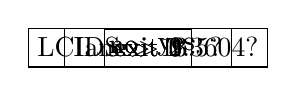
\begin{tikzpicture}[
    node/.style={%
      draw,
      rectangle,
    },
  ]

    \node [node] (A) {IDS $>$ 13.5?};
    \path (A) ++(-135:\nodeDist) node [node] (B) {exit 1};
    \path (A) ++(-45:\nodeDist) node [node] (C) {LCIanx $>$ 0.3604?};
    \path (C) ++(-135:\nodeDist) node [node] (D) {exit 2};
    \path (C) ++(-45:\nodeDist) node [node] (E) {exit 3};

    \draw (A) -- (B) node [left,pos=0.25] {no}(A);
    \draw (A) -- (C) node [right,pos=0.25] {yes}(A);
    \draw (C) -- (D) node [left,pos=0.25] {no}(A);
    \draw (C) -- (E) node [right,pos=0.25] {yes}(A);
\end{tikzpicture}
	\captionsource{Árbol de decisión}{\fuentePropia}
	\label{fig:decision-tree}
\end{figure}


\subsubsection*{Máquinas de vectores de soporte (SVM)}
Las máquinas de vectores de soporte o SVM (del inglés \ingles{Support Vector Machine}) son un conjunto de algoritmos de aprendizaje supervisado que se enfocan en resolver problemas de clasificación, regresión y agrupamiento. La SVM destinada para clasificación, es un clasificador lineal binario que busca encontrar un hiperplano que separe de forma óptima un conjunto de datos, maximizando la distancia entre las dos clases.


\begin{figure}[H]
	\centering
	\begin{tikzpicture}[&gt;=stealth']
  % Draw axes
  \draw [&lt;-&gt;,thick] (0,5) node (yaxis) [above] {$y$}
        |- (5,0) node (xaxis) [right] {$x$};
  % draw line
  \draw (0,-1) -- (5,4); % y=x-1
  \draw[dashed] (-1,0) -- (4,5); % y=x+1
  \draw[dashed] (2,-1) -- (6,3); % y=x-3
  % \draw labels
  \draw (3.5,3) node[rotate=45,font=\small] 
        {$\mathbf{w}\cdot \mathbf{x} + b = 0$};
  \draw (2.5,4) node[rotate=45,font=\small] 
        {$\mathbf{w}\cdot \mathbf{x} + b > 1$};
  \draw (4.5,2) node[rotate=45,font=\small] 
        {$\mathbf{w}\cdot \mathbf{x} + b < -1$};
  % draw distance
  \draw[dotted] (4,5) -- (6,3);
  \draw (5.25,4.25) node[rotate=-45] {$\frac{2}{\Vert \mathbf{w} \Vert}$};
  \draw[dotted] (0,0) -- (0.5,-0.5);
  \draw (0,-0.5) node[rotate=-45] {$\frac{b}{\Vert \mathbf{w} \Vert}$};
  \draw[-&gt;] (2,1) -- (1.5,1.5);
  \draw (1.85,1.35) node[rotate=-45] {$\mathbf{w}$};
  % draw negative dots
  \fill[red] (0.5,1.5) circle (3pt);
  \fill[red]   (1.5,2.5)   circle (3pt);
  \fill[black] (1,2.5)     circle (3pt);
  \fill[black] (0.75,2)    circle (3pt);
  \fill[black] (0.6,1.9)   circle (3pt);
  \fill[black] (0.77, 2.5) circle (3pt);
  \fill[black] (1.5,3)     circle (3pt);
  \fill[black] (1.3,3.3)   circle (3pt);
  \fill[black] (0.6,3.2)   circle (3pt);
  % draw positive dots
  \draw[red,thick] (4,1)     circle (3pt); 
  \draw[red,thick] (3.3,.3)  circle (3pt); 
  \draw[black]     (4.5,1.2) circle (3pt); 
  \draw[black]     (4.5,.5)  circle (3pt); 
  \draw[black]     (3.9,.7)  circle (3pt); 
  \draw[black]     (5,1)     circle (3pt); 
  \draw[black]     (3.5,.2)  circle (3pt); 
  \draw[black]     (4,.3)    circle (3pt); 
\end{tikzpicture}
	\captionsource{SVM}{\fuentePropia}
	\label{fig:svm}
\end{figure}

\subsubsection*{Perceptrón}

\begin{figure}[H]
	\centering
	% Multilayer perceptron
\usetikzlibrary{positioning}

\tikzstyle{inputNode}=[draw,circle,minimum size=10pt,inner sep=0pt]
\tikzstyle{stateTransition}=[-stealth, thick]

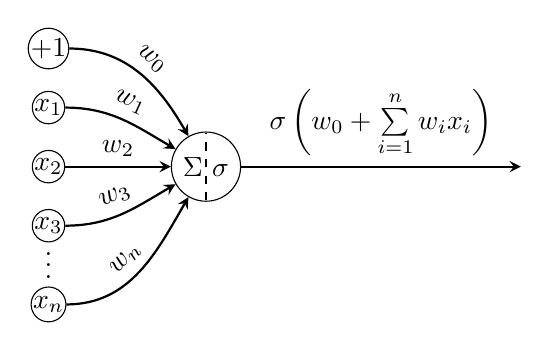
\begin{tikzpicture}
    \node[draw,circle,minimum size=25pt,inner sep=0pt] (x) at (0,0) {$\Sigma$ $\sigma$};

    \node[inputNode] (x0) at (-2, 1.5) {$\tiny +1$};
    \node[inputNode] (x1) at (-2, 0.75) {$\tiny x_1$};
    \node[inputNode] (x2) at (-2, 0) {$\tiny x_2$};
    \node[inputNode] (x3) at (-2, -0.75) {$\tiny x_3$};
    \node[inputNode] (xn) at (-2, -1.75) {$\tiny x_n$};

    \draw[stateTransition] (x0) to[out=0,in=120] node [midway, sloped, above] {$w_0$} (x);
    \draw[stateTransition] (x1) to[out=0,in=150] node [midway, sloped, above] {$w_1$} (x);
    \draw[stateTransition] (x2) to[out=0,in=180] node [midway, sloped, above] {$w_2$} (x);
    \draw[stateTransition] (x3) to[out=0,in=210] node [midway, sloped, above] {$w_3$} (x);
    \draw[stateTransition] (xn) to[out=0,in=240] node [midway, sloped, above] {$w_n$} (x);
    \draw[stateTransition] (x) -- (4,0) node [midway,above] {$\sigma\left(w_0 + \sum\limits_{i=1}^{n}{w_ix_i}\right)$};
    \draw[dashed] (0,-0.43) -- (0,0.43);
    \node (dots) at (-2, -1.15) {$\vdots$};
    
\end{tikzpicture}

	\captionsource{Perceptrón}{\fuentePropia}
	\label{fig:perceptron}
\end{figure}

\begin{equation}
 \pmb{\mu_1} = \begin{bmatrix}0\\0\\...\\0\end{bmatrix}
\end{equation}

\subsubsection*{Perceptrón multicapa}

\begin{figure}[H]
	\centering
	% Multilayer perceptron
\usetikzlibrary{positioning}

\tikzstyle{inputNode}=[draw,circle,minimum size=10pt,inner sep=0pt]
\tikzstyle{stateTransition}=[-stealth, thick]

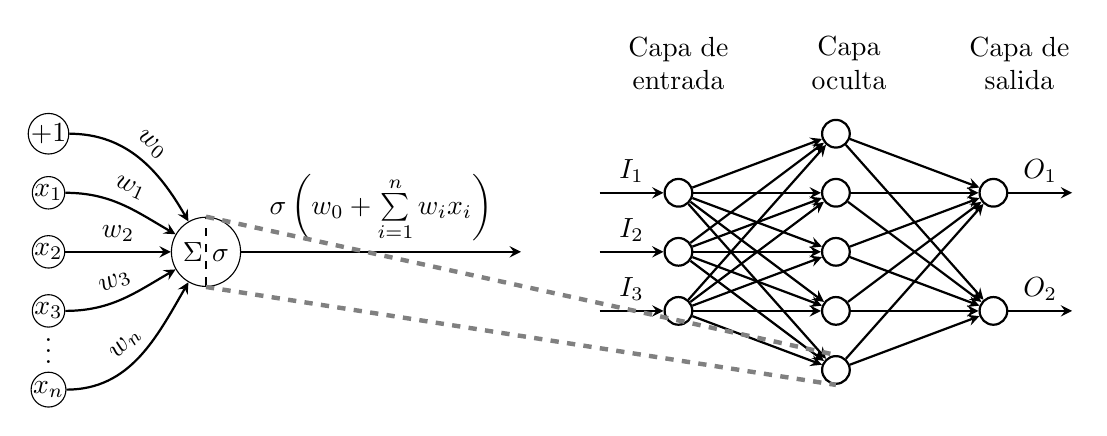
\begin{tikzpicture}
    \node[draw,circle,minimum size=25pt,inner sep=0pt] (x) at (0,0) {$\Sigma$ $\sigma$};

    \node[inputNode] (x0) at (-2, 1.5) {$\tiny +1$};
    \node[inputNode] (x1) at (-2, 0.75) {$\tiny x_1$};
    \node[inputNode] (x2) at (-2, 0) {$\tiny x_2$};
    \node[inputNode] (x3) at (-2, -0.75) {$\tiny x_3$};
    \node[inputNode] (xn) at (-2, -1.75) {$\tiny x_n$};

    \draw[stateTransition] (x0) to[out=0,in=120] node [midway, sloped, above] {$w_0$} (x);
    \draw[stateTransition] (x1) to[out=0,in=150] node [midway, sloped, above] {$w_1$} (x);
    \draw[stateTransition] (x2) to[out=0,in=180] node [midway, sloped, above] {$w_2$} (x);
    \draw[stateTransition] (x3) to[out=0,in=210] node [midway, sloped, above] {$w_3$} (x);
    \draw[stateTransition] (xn) to[out=0,in=240] node [midway, sloped, above] {$w_n$} (x);
    \draw[stateTransition] (x) -- (4,0) node [midway,above] {$\sigma\left(w_0 + \sum\limits_{i=1}^{n}{w_ix_i}\right)$};
    \draw[dashed] (0,-0.43) -- (0,0.43);
    \node (dots) at (-2, -1.15) {$\vdots$};
    \node[inputNode, thick] (i1) at (6, 0.75) {};
    \node[inputNode, thick] (i2) at (6, 0) {};
    \node[inputNode, thick] (i3) at (6, -0.75) {};
    
    \node[inputNode, thick] (h1) at (8, 1.5) {};
    \node[inputNode, thick] (h2) at (8, 0.75) {};
    \node[inputNode, thick] (h3) at (8, 0) {};
    \node[inputNode, thick] (h4) at (8, -0.75) {};
    \node[inputNode, thick] (h5) at (8, -1.5) {};
    
    \node[inputNode, thick] (o1) at (10, 0.75) {};
    \node[inputNode, thick] (o2) at (10, -0.75) {};
    
    \draw[stateTransition] (5, 0.75) -- node[above] {$I_1$} (i1);
    \draw[stateTransition] (5, 0) -- node[above] {$I_2$} (i2);
    \draw[stateTransition] (5, -0.75) -- node[above] {$I_3$} (i3);
    
    \draw[stateTransition] (i1) -- (h1);
    \draw[stateTransition] (i1) -- (h2);
    \draw[stateTransition] (i1) -- (h3);
    \draw[stateTransition] (i1) -- (h4);
    \draw[stateTransition] (i1) -- (h5);
    \draw[stateTransition] (i2) -- (h1);
    \draw[stateTransition] (i2) -- (h2);
    \draw[stateTransition] (i2) -- (h3);
    \draw[stateTransition] (i2) -- (h4);
    \draw[stateTransition] (i2) -- (h5);
    \draw[stateTransition] (i3) -- (h1);
    \draw[stateTransition] (i3) -- (h2);
    \draw[stateTransition] (i3) -- (h3);
    \draw[stateTransition] (i3) -- (h4);
    \draw[stateTransition] (i3) -- (h5);
    
    \draw[stateTransition] (h1) -- (o1);
    \draw[stateTransition] (h1) -- (o2);
    \draw[stateTransition] (h2) -- (o1);
    \draw[stateTransition] (h2) -- (o2);
    \draw[stateTransition] (h3) -- (o1);
    \draw[stateTransition] (h3) -- (o2);
    \draw[stateTransition] (h4) -- (o1);
    \draw[stateTransition] (h4) -- (o2);
    \draw[stateTransition] (h5) -- (o1);
    \draw[stateTransition] (h5) -- (o2);
    
    %Input layer
    \node[above=of i1, align=center] (l1) {Capa de \\ entrada};
    %Hidden Layer
    \node[right=2.3em of l1, align=center] (l2) {Capa \\ oculta};
    %Output Layer
    \node[right=2.3em of l2, align=center] (l3) {Capa de \\ salida};
    
    \draw[stateTransition] (o1) -- node[above] {$O_1$} (11, 0.75);
    \draw[stateTransition] (o2) -- node[above] {$O_2$} (11, -0.75);
    
    \path[dashed, double, ultra thick, gray] (x.north) edge[bend left=0] (h5.north);
    \path[dashed, double, ultra thick, gray] (x.south) edge[bend right=0] (h5.south);
\end{tikzpicture}

	\captionsource{Perceptrón multicapa}{\fuentePropia}
	\label{fig:multilayer-perceptron}
\end{figure}

\subsubsection*{Na\"ive Bayes}
El clasificador Na\"ive Bayes, también conocido como clasificador bayesiano, es un clasificador probabilístico basado en el teorema de Bayes descrito en la \ec{eq:naive-bayes}, donde $P(A|B)$ es la probabilidad de la hipotesis

\begin{equation}
 P(A|B) = \frac{P(A) \cdot P(B|A)}{P(B)}
 \label{eq:naive-bayes}
\end{equation}


\subsection{Minería de datos educacional}
La minería de datos utiliza una combinación de bases de conocimientos explícita, conocimientos analíticos complejos y conocimiento de campo para descubrir las tendencias y los patrones ocultos, estas tendencias y patrones forman la base de los modelos predictivos que permiten a los analistas realizar nuevas observaciones de los datos existentes \parencite{luan2002data}. La gran cantidad de información generada hoy en día por los estudiantes permite que la minería de datos obtenga datos relevantes y, a través de métodos estadísticos y otras herramientas relacione la información para conocer si el proceso de enseñanza aprendizaje ha dado resultados positivos. 

\textcite[p.~9]{mining2012enhancing} define la minería de datos educacional (MDE, desde ahora en adelante) como “la teoría que desarrolla métodos, aplica técnicas estadísticas y de aprendizaje automático para analizar los datos recogidos durante el proceso de la enseñanza y aprendizaje” \footnote{\traduccionlibre}. Actualmente, los usos más generales que se le están dando a la MDE básicamente se enfocan en mejorar la estructura del conocimiento y determinar el apoyo pedagógico al estudiante.
\section{Estado del arte}
\label{sec:estado_arte}
%TODO: fix
El propósito de esta sección es presentar los últimos trabajos realizados en la línea de investigación de la alfabetización informacional, comportamiento de estudiantes, minería de datos educacional y predicción del desempeño en tareas de estudiantes. La búsqueda de estos trabajos considera: la exploración de trabajos con estudios que midan experiencia de usuario y/o medidas de rendimiento en la utilización de interfaces no-tradicionales operadas con el cuerpo para la realización de actividades en distintos contextos.

\subsection{Alfabetización informacional}
%La enseñanza de competencias informacionales o alfabetización informacional, se imparte principalmente por bibliotecas universitarias, y en un menor grado en la etapa escolar obligatoria. A pesar de esto, algunas universidades suelen considerar las competencias informacionales como un requisito de entrada, aprendidas antes de iniciar los estudios universitarios, variando su importancia según los principios de cada carrera. Un ejemplo de esto, es la investigación de Weiner (2014) en la cual se utilizaron encuestas para determinar las competencias informacionales de interés en los programas de colleges y universitarios. En el trabajo de Smith et al. (2013) queda de manifiesto que la alfabetización informacional en enseñanza escolar no necesariamente está vinculada con las reales necesidades universitarias. En dicho trabajo, un grupo de estudiantes canadienses de último año, pertenecientes a escuelas que desarrollan las competencias informacionales, fueron sometidos a un test universitario que mide estas competencias. Los resultados evidencian que los alumnos no se están graduando con el adecuado nivel de alfabetización informacional. 

%A nivel nacional, la enseñanza de estas competencias se realiza principalmente por parte de las bibliotecas universitarias, por lo cual, Marzal y Sauriana (2015) realizan un análisis de la situación actual de los cursos y políticas de alfabetización informacional de las bibliotecas pertenecientes al Consejo Nacional de Educación. Se concluye que no existe uniformidad en las definiciones y marcos teóricos utilizados. Por otro lado, los estudiantes universitarios chilenos presentan dificultades con las competencias informacionales (p. ej. aprenderlas, pero no utilizarlas), hecho que se vio reflejado por el estudio interno realizado por la Universidad de Playa Ancha (Urra & Castro, 2016) sobre el impacto de la enseñanza de la alfabetización informacional en dicha universidad. Una de las posibles causas de por qué los estudiantes tienen dificultades es el hecho de que en los colegios no se prioriza la generación de conocimiento, sino la reiteración de la información.  

%En Finlandia, la enseñanza de alfabetización informacional también inicia en las bibliotecas académicas. Durante los años 1990 a 2002 tuvo efecto la transición de educar en el uso de los sistemas de bibliotecas a la enseñanza de competencias informacionales (Sinikara & Järveläinen, 2003). A razón de esto, los primeros estudios y cambios curriculares se enfocaron en este nivel. Por ejemplo, el proyecto “Standardizing the management of the information literacy 2001–2003” de la biblioteca de la Universidad de Helsinki realizó una traducción al finlandés de los estándares de alfabetización internacional propuestos por la ARCL (Asociación de Bibliotecas Universitarias y de Investigación) mientras que en 2004 las bibliotecas universitarias lanzaron un proyecto nacional para la creación de un currículum universitario de competencias informacionales (Kämäräinen & Saarti, 2013).

%El siguiente paso en Finlandia fue enfocar los estudios y proyectos al nivel de secundaria. El trabajo realizado por Sormunen, Alamettälä, y Heinström (2013) es ejemplo de la incorporación de las competencias informacionales de forma transversal al proceso educativo, bajo el enfoque de enriquecer el aprendizaje al momento de realizar tareas grupales en el aula, aplicado a la escritura de artículos en clases de historia y literatura. Por otro lado, Alamettälä (2015) propone un plan de trabajo para la enseñanza formal de alfabetización informacional en los primeros niveles de la educación secundaria finlandesa. 

%Actualmente, a nivel educacional primario, tres universidades finlandesas (University of Tampere, University of Jyväskylä y University of Turku) en conjunto con dos universidades chilenas (Universidad de Santiago de Chile y Pontificia Universidad Católica) están realizando una intervención en el aula respecto las competencias informacionales en quinto y sexto año básico (CONICYT, 2015), para establecer un marco de enseñanza de estas competencias, que pueda derivar en propuestas públicas y cambios curriculares. Puntualmente el trabajo realizado por Sormunen, González-Ibáñez y Kiili (2017) introduce nuevas formas de evaluar las competencias de investigación en línea (online inquiry) específicamente en búsqueda, evaluación, recolección y síntesis de la información.


A nivel nacional, la enseñanza de las competencias de investigación se realizan principalmente por parte de las bibliotecas universitarias, por lo cual, \textcite{marzal2015diagnostico} realizan un análisis de la situación actual de los cursos y políticas de alfabetización informacional de las bibliotecas pertenecientes al Consejo Nacional de Educación. Se concluye que no existe uniformidad en las definiciones y marcos teóricos utilizados. Por otro lado, los estudiantes universitarios chilenos presentan dificultades con las competencias informacionales, tales como aprenderlas, pero no utilizarlas, hecho que se vio reflejado por el estudio interno realizado por la Universidad de Playa Ancha \parencite{urra2016alfabetizacion} sobre el impacto de la enseñanza de la alfabetización informacional en dicha universidad. Una de las posibles causas de por qué los estudiantes tienen dificultades es el hecho de que en los colegios no se prioriza la generación de conocimiento, sino la reiteración de la información.

A nivel internacional, tres universidades finlandesas (University of Tampere, University of Jyv\"askyl\"a y University of Turku) en conjunto con dos universidades chilenas (Universidad de Santiago de Chile y Pontificia Universidad Católica) están realizando una intervención en el aula respecto las competencias informacionales en quinto y sexto año básico (CONICYT, 2015), para establecer un marco de enseñanza de estas competencias, que pueda derivar en propuestas públicas y cambios curriculares. Puntualmente, el trabajo realizado por \textcite{gonzalez2017neurone} introduce nuevas formas de evaluar las competencias de investigación en línea específicamente en búsqueda, evaluación, recolección y síntesis de la información.

\subsection{Comportamiento de búsqueda de información de estudiantes}

%Agregar esto:  Sormunen, González-Ibáñez y Kiili (2017) introduce nuevas formas de evaluar las competencias de investigación en línea (online inquiry) específicamente en búsqueda, evaluación, recolección y síntesis de la información.   

Con la incorporación de herramientas digitales en la enseñanza escolar es necesario evaluar su aporte en el aprendizaje. En general, en la evaluación se analizan las mediciones respecto a los datos proporcionados por los estudiantes, ya sea de forma directa, como cuestionarios o indirecta, como datos generados al utilizar un sistema computacional pero con previa autorización del estudiante.

\textcite{henrie2015measuring} clasifica los datos generados por los estudiantes en un sistema computacional en tres categorías: comportamiento, cognitivas y emocionales. El comportamiento de los estudiantes es una de las más estudiadas, en esta categoría se estudian las variables cuantitativas: resultados de consultas realizadas en un motor de búsqueda, teclas presionadas, rastreo ocular, tareas de búsqueda, esfuerzo (intentos por finalizar tareas asignadas), participación, tiempos de permanencia o de respuestas y uso de sitios \ingles{web}, entre otros. Tomando tiempos de permancencia y el uso de sitios, \textcite{Shah2016} presenta diversas métricas para evaluar el rendimiento de la búsqueda de información, en base a las distintas acciones hechas por usuarios. Tales métricas se usan con el objetivo de pronosticar la probabilidad de un usuario de tener éxito en el futuro, en base a su desempeño actual. 

Los trabajos de \textcite{hwang2008novel} y \textcite{tu2008eighth} son ejemplos de la creación de sistemas para la recolección de registros de datos de estudiantes. La información recopilada varía desde respuestas directas a preguntas, historial de navegación, tiempos, entradas de teclado, marcación de páginas, hasta reformulación de la consulta, entre otros. El enfoque del trabajo de \textcite{hwang2008novel} fue ayudar a los profesores a evaluar de forma indirecta el desempeño de los estudiantes y realizar intervenciones en el aprendizaje. En este sistema el resumen de la navegación y las respuestas de los estudiantes eran visibles para los profesores, permitiendo distinguir indicadores del comportamiento \ingles{web} de los niños. En cambio, el estudio de \textcite{tu2008eighth} se realizó para determinar la influencia de factores externos en el proceso de búsqueda de información de estudiantes de básica, específicamente centrado en la forma en que las creencias epistemológicas y otros factores externos se relacionan con los resultados del proceso de búsqueda de información en un entorno \ingles{web}. Para lograrlo se realizó una mezcla entre cuestionarios, tareas de búsqueda específica y análisis de los datos generados por los estudiantes durante su navegación. El trabajo más reciente en el área, es la aplicación web NEURONE \parencite{gonzalez2017neurone} acrónimo de \ingles{oNlinE inquiry expeRimentatiON systEm}, es un sistema de apoyo para la evaluación de competencias de investigación en línea para estudiantes de enseñanza básica, en base a los requerimientos del proyecto “\ingles{Enhancing learning and teaching future competences of online inquiry in multiple domains} (iFuCo)” \parencite{sormen2017performance}, para registrar las acciones realizadas por los estudiantes durante una tarea de investigación. 

Siguiendo este tipo de análisis sobre datos generados por estudiantes, en la prueba internacional PISA \parencite{PISA} se analizaron los registros de la navegación en un sitio \ingles{web} ficticio, con múltiples hipervínculos internos. El sitio estaba dividido en diferentes páginas unidas por \ingles{links}, clasificados en tres niveles, siendo las de nivel 1 las más fáciles de acceder (variados hipervínculos conducían a éstas), en cambio, la ruta para llegar a las de nivel 3 era específica. Para contestar las preguntas de comprensión lectora era necesario encontrar la página con la información necesaria, la cual, dependiendo de su nivel (1 a 3) podía transformar la tarea de una navegación simple a una compleja. El objetivo de el análisis fue determinar qué tan fluida es la lectura en línea, los diferentes desempeños de los estudiantes y la persistencia al tratar de responder.


\subsection{Minería de datos educacional}

%TODO: Expandir esto
%\textcite{baker2010data} desarrolló un modelo de predicción usando datos recopilados automáticamente de interacciones entre estudiantes y el \ingles{software} como variables de predicción, y después validando la precisión del modelo al ser generalizado a más estudiantes y contextos. Entonces fueron capaces de estudiar sus avances en el conjunto completo de datos.

Actualmente, la aplicación de la MDE radica en universidades, tales como Paul Smith’s College, la cual utiliza sus datos históricos para mejorar las tasas de retención de alumnos \parencite{bichsel2012analytics}. En este contexto, University of Georgia desarrolló un modelo para predecir la tasa de graduación y abandono estudiantil, el cual se alimenta en base la información recopilada \parencite{morris2005predicting}. Finalmente, la Purdue University han usado MDE para determinar que la evaluación en etapas tempranas y de forma frecuente permite cambiar los hábitos de los estudiantes con calificaciones bajo la media en cursos introductorios, en base a este trabajo, el mismo equipo de investigación desarrollo un sistema de alerta académica temprana para saber el desempeño de los estudiantes \parencite{baepler2010academic}. 

\textcite{merceron2005educational} establece cómo los algoritmos de minería de datos pueden escoger información pedagógica importante. El conocimiento obtenido ayuda a mejorar el cómo administrar la clase, como el alumno aprende, y cómo proporcionar retroalimentación a los alumnos. Basado en este trabajo, \textcite{abdullah2014students} realiza un sistema de predicción del rendimiento de los estudiantes basado en la actividad actual y mediciones anteriores clasificando cuales estudiantes rendirán bien y los que no. 

\textcite{chen2008integrated} evalúa el rendimiento académico de estudiantes de pregrado estudiando datos académicos del Departamento de Ciencias de la Computación de National Defence Univiersity of Malaysia (NUDM) utilizando una combinación de técnicas de minería de datos, como ANN (\ingles{Artificial Neural Network}) y árboles de decisión como un método de clasificación con el que se producen ocho reglas para la identificación automática de los estilos cognitivos de los estudiantes basados en sus patrones de aprendizaje. Los hallazgos obtenidos se aplicaron para desarrollar un modelo que pueda apoyar el desarrollo de programas educativos \ingles{web}.

\textcite{moreno2009data} predice la probabilidad de que los estudiantes de acuerdo a sus registros académicos históricos fallen en un curso \ingles{online} en Moodle\footnote{https://moodle.org/} haciendo uso de las técnicas de maximización, el método de agrupamiento K-means y X-means, usando el \ingles{software} WEKA.

%Dickerson \& Hazelton (2012) exploran y ponen en práctica las técnicas de minería de datos para crear un nuevo circuito de retroalimentación hacia los profesores para la evaluación de programas y la adaptación sistemática a los cambios que requiere el sector empresarial de sus estudiantes.

%Guruler \& Istanbullu (2014) evaluan y desarrollan un enfoque basado en datos relacionados con la mejora del rendimiento de los estudiantes universitarios mediante la aplicación de técnicas incluidas en el ámbito del "Descubrimiento de Conocimiento en Bases de Datos" (conocido como KDD, las iniciales de \ingles{Knowledge Discovery in Databases}), combinado con minería de datos. 

%\textcite{sarala2015empirical} discute las aplicaciones de la minería de datos en instituciones educativas, para extraer la información útil de grandes conjuntos de datos (\ingles{datasets}), y proporciona herramientas analíticas para ver y utilizar esta información para tomar decisiones basadas en ejemplos de la vida real.

%\textcite{kalpana2014intellectual} analiza el rendimiento de los estudiantes de la facultad de ingeniería de conducted the students’ performance analysis on the graduate students’ data collected from the Villupuram college of Engineering and Technology. The data included five year period and applied clustering methods on the data to overcome the problem of low score of graduate students, and to raise students academic performance .

%\textcite{suyal2014quality} aplica técnicas de asociación y clasificación para predecir el rendimiento académico de los estudiantes applied the association and classification rule to identify the students’ performance. They mainly focused to find the students who need special attention to reduce failure rate . 

 


\subsection{Predicción del desempeño estudiantil}
La predicción está enfocada en pronosticar el desempeño estimando valores desconocidos de variables que caracterizan al estudiante. Estos valores normalmente corresponden al rendimiento, conocimiento o calificaciones. También se utiliza para detectar estilos de aprendizaje, predecir si contestará correctamente una pregunta, modelar los cambios en el conocimiento al adquirir un nuevo aprendizaje y determinar variables del aprendizaje no observables en la conducta en línea de los estudiantes \parencite{romero2010educational}. 

En general, el enfoque es detectar de forma temprana quienes probablemente tendrán un bajo desempeño o encontrar los indicadores que permitan identificar a estos alumnos de tal forma que el profesor o la entidad educacional correspondiente pueda intervenir a tiempo y prevenir por ejemplo la deserción escolar. 

En esta línea, \textcite{antunes2010anticipating} se centró en anticipar el fracaso de los estudiantes lo más pronto posible en cursos de fundamentos de la programación. Se utilizó la información de los estudiantes universitarios (12 atributos observables y 4 de calificaciones) que han cursado dicha asignatura a lo largo de cinco años. Con el algoritmo J48 se construyeron tres clasificadores bajo distintos enfoques para determinar reglas de decisión que permitan predecir el fracaso. Por otro lado, el estudio realizado por \textcite{kumar2016predicting} identificó a los estudiantes con mayor probabilidad de aprobar el examen final de una carrera de ingeniería. En base a atributos numéricos como las notas de secundaria y de semestres previos al examen, en conjunto a variables demográficas tales como, género, estado civil, ocupaciones de los padres, entre otros, se realizó la predicción del desempeño de los estudiantes, siendo los algoritmos J48 y REPtree los con mejor desempeño.

A nivel escolar, \textcite{marquez2013predicting} buscaron predecir el bajo rendimiento escolar y asociarlo con las causas de la deserción escolar o repitencia. Realizaron una investigación con estudiantes mexicanos de 15 y 16 años, con el objetivo de determinar los factores más influyentes y las razones que llevan al fracaso, e identificar a los estudiantes que muestran estas características para ofrecerles la ayuda correspondiente. Se consideraron atributos socioeconómicos, personales, sociales, familiares, escolares y calificaciones, haciendo uso de diez algoritmos de clasificación tradicionales, cinco para la construcción de árboles de decisión (J48, RandomTree, Reptree, SimpleCart y ADtree) y cinco para la generación de reglas asociación (JRIP, NNge, OneR, Prism y Ripdor). Además, crearon un algoritmo utilizando programación genética gramatical para predecir si un estudiante aprueba o reprueba. Los resultados muestran que con este algoritmo evolucionado se obtienen resultados tan precisos como con los algoritmos tradicionales, pero con menos reglas y condiciones por regla, permitiendo así reducir el número de características, y utilizarlas para detectar a los estudiantes con mayor tendencia a repetir el año escolar.

\textcite{shamsi2016comparative} se realiza un análisis comparativo de distintas técnicas de clasificación (Na\"ive Bayes, LibSVM, J48, Random Forest y JRIP) aplicado a determinar los factores claves que afectan el rendimiento en estudiantes de ingeniería en la India, bajo la premisa de que una inapropiada educación primaria y secundaria repercute en desempeño de la educación superior de estos estudiantes. Se consideraron 34 parámetros, en su mayoría variables descriptivas asociadas al entorno familiar. Los resultados obtenidos mostraron que Na\"ive Bayes es el más exacto para predecir un mal desempeño y JRIP el más preciso en la predicción de las calificaciones, junto con entregar los factores que afectan el rendimiento en un set de reglas.

%\subsection{Técnicas utilizadas en la minería de datos educacional}

%Khan \& Choi (2014) a través de un árbol de decisión y algoritmos procesan los datos de los estudiantes para calcular las posibilidades de ganar una beca en función de su grado de semestre, la ubicación del alumno en clase, la cantidad máxima y mínima de horas de crédito tomadas y permitidas y las actividades extracurriculares. 



%TODO: Profundizar
%Dutt es un review
%\textcite{dutt2015clustering} consolida las variantes de algoritmos de clustering aplicados al contexto de MDE. Además, simplifica el diseño los sistemas que aprenden de los datos, utilizando técnicas y algoritmos de minería de datos, tales como, clustering, clasificación y predicción.

\textcite{lahtinen2005study} estudia las dificultades de aprender programación con el objetivo de crear material adecuado para introducir el curso a los estudiantes utilizando el método de agrupamiento \ingles{K-means} y \ingles{Hierarchical clustering} (más conocido como Ward's \ingles{clustering}, a través de este estudio se obtuvo las dificultades que sufren los estudiantes al momento de enfrentar tareas de programación. Basado en este trabajo \textcite{akinola2012data} aplica ANN para predecir el resultado de los cursos de programación en estudiantes de pregrado basados en su historial académico, los resultados de este estudio muestran que los estudiantes con un conocimiento a priori de física y matemática tienen mejor desempeño en los cursos que el resto.

%TODO: FIX THIS
\textcite{borkar2014attributes} evalúa el rendimiento de los estudiantes, donde selecciona algunos atributos mediante minería de datos, haciendo uso de una red neuronal multicapa perceptrón y usando una validación cruzada selecciona las características más influyentes, estableciendo las reglas necesarias para poder detectar las características necesarias para poder predecir el rendimiento de los estudiantes. Basado en los métodos propuestos y el mismo conjunto de datos de este trabajo, \textcite{jayakameswaraiah2014study} compara los métodos de perceptrón multicapa, Na\"ive Bayes, SMO y J48 con el objetivo de obtener el mejor algoritmo de clasificación y predicción entre todos ellos. De todos los métodos comparados, el método de perceptrón multicapa obtuvo un \ingles{accuracy} de 75\%.


%fuente: http://www.ijiee.org/vol5/513-F1002.pdf
%[33] To analyze the web log data files of a Leaning Management System (LMS). Markov Clustering (MCL) algorithm for clustering the students‟ activity and a SimpleKMeans algorithm for clustering the courses. The data are from the spring semester of 2009 from the Department of Information management and involve 1199 students and 39 different courses. The data are in ASCII form and are obtained from the Apache server log file

% Sacar referencias de: http://ieeexplore.ieee.org.ezproxy.usach.cl/stamp/stamp.jsp?tp=&arnumber=7684167
%Sheik and Gadage have done the analysis related to the student learning behavior by using different data mining models, namely classification, clustering, decision tree, sequential pattern mining and text mining. They used open source tools such as KNIME (Konstanz Information Miner), RAPIDMINER, WEKA, CARROT, ORANGE, RProgramming, and iDA. These tools have different compatibilities and it provided an insight into the prediction and evaluation [2]

%Mythili M S and Shanavas A R applied classification algorithms to analyze and evaluate school students performance using weka. They came with various classification algorithms, namely J48, Random Forest, Multilayer perception, IBI and decision table with the data collected from the student management system [3]. 

%Osmanbegovic and Suljic conducted a study for investigating students’ future performance in the end semester results at the University of Tuzla. They considered 11 factors and used classification model with highest accuracy for naive Bayes [5]

%Noah, Barida and Egerton conducted a study to evaluate students’ performance by grouping the grading into various classes using CGPA. They used different methods like Neural network, Regression and K-means to identify the weak performers for the purpose of performance improvement [7]. 


%\subsubsection*{Identificación de factores}
\textcite{borkar2013predicting} sugiere un método de evaluación del rendimiento de los estudiantes usando reglas asociativas de minería de datos, estimando el resultado de los estudiantes basado en la asistencia a sus cursos y su avance académico. Basado en este trabajo, \textcite{shazmeen2013performance} evalúa el rendimiento de diferentes algoritmos de clasificación y análisis predictivo, proponiendo técnicas de preprocesamiento de datos para lograr mejores resultados.

\textcite{oskouei2014predicting} identifica los factores que afectan el rendimiento de los estudiantes en diferentes países, y aplica técnicas de clasificación y predicción para mejorar la precisión de las predicciones de los resultados de los estudiantes. Los resultados muestran que los factores de género, entorno familiar, nivel de educación de los padres, y el estilo de vida afectan el rendimiento académico de los estudiantes independiente del país.

\textcite{rgonzalez2012} utiliza

% Ya citado
%\textcite{Shah2016} utiliza

\textcite{rgonzalez2015} utiliza

\textcite{hassan2013beyond} utiliza
A pesar de que el número de clics es un atributo de interés en varios estudios, sobre todo 
combinados con otros atributos, por ejemplo, con reformulaciones de consulta (Hassan et al., 
2013), en esta investigación, se descartó rápidamente por afectar negativamente los resultados 
de la clasificación. Los sitios web utilizados no contienen hipervínculos, ni despliegues de menú 
con clics derechos, lo que podría explicar porque esta variable sólo generó ruido   


%\parencite{marquez2013predicting}

%En el trabajo de Chen et al. (2001) se hace una correlación entre el el movimiento de los ojos (medidos con un sensor de rastreo ocular) y el movimiento del ratón al navegar en la web. Dicho estudio muestra que 84% de las veces que una región de la ventana es visitada por el cursor del ratón, también es mirada por el usuario. Además el 88% de las regiones que son miradas por el usuario, tampoco son visitadas por el cursor del ratón. En síntesis, es posible afirmar que se puede utilizar la posición del ratón como un indicador de la mirada del usuario en la pantalla de forma relativamente precisa, además de ser no invasiva y ser de bajo costo.

%Tanto White & Drucker (2007) como Odijk et al. (2015) detallan que el análisis de los patrones de interacción de los usuarios dentro de ambientes de búsqueda web permiten revelar diferentes comportamientos, y por ende, diferentes estilos de procesar y asimilar la información a la hora de ejecutar tareas de búsqueda. Para realizar este análisis se debe llevar un registro de la sesión y páginas visitadas por el usuario durante la búsqueda.

%En Jiang & Ni (2016) se hace alusión a la reformulación de consultas de búsqueda web como elemento a considerar a la hora de analizar la efectividad de la búsqueda y el refinamiento que ésta alcanza a través del “ensayo y error”. Dicho análisis puede ser llevado a cabo rastreando la actividad del teclado (keystrokes) y/o la actividad del formulario de búsqueda.


%TODO: ¿Que es un buen modelo?
%FULL REFERENCE:
%“Un buen modelo cognitivo del conocimiento del estudiante debe ser capaz de predecir las diferencias en la dificultad de una tarea, o cómo es que el aprendizaje es transferido de tarea en tarea” (Koedinger et al. , 2015, pág. 339). Las investigaciones en minería de datos educacional se realizan mayoritariamente en aprendizaje online y en casos puntuales en educación superior, por lo que es limitada la información respecto a educación primaria o secundaria, sobre todo en lo que concierne a predicción de errores y fracaso escolar (Márquez-Vera et al., 2013). 
%\textcite{koedinger2015data} define que un buen modelo cognitivo de un estudiante debe ser capaz de predecir las diferencias en la dificultad de una tarea, y como el aprendizaje es transferido de tarea en tarea.

%Baradwaj and pal described data mining techniques that help in early identification of student dropouts and students who need special attention. Here they used a decision tree by using information like attendance, class test, semester and assignment marks [8]. 

%Jeevalatha, Ananthi, and Saravana Kumar presented a case study on performance analysis for placement selection for undergraduate students. They applied decision tree algorithm by considering the factors like HSC, UG marks and communication skills [9]. 

%En esta sección se presenta el estado del arte que da soporte a este trabajo, el cual comprende en primer lugar el estudio del comportamiento de estudiantes. En segundo lugar, técnicas de minería de datos y plataformas de aprendizaje de máquina aplicada al contexto educacional.

%\subsection{Plataformas de aprendizaje de máquinas aplicadas al contexto educacional}

%Cuando se aplica minería de datos en instituciones educativas, la disciplina se conoce como minería de datos educacional (MDE, desde ahora en adelante).

%La MDE es una disciplina en evolución que usa tecnologías informáticas, como son almacenes de datos y herramientas de inteligencia de negocios para descubrir tendencias y patrones sobre datos educacionales. El conocimiento que la MDE genera apoya a las autoridades de centros de educación en la toma de decisiones oportunas, y a los profesores para analizar el comportamiento y aprendizaje de sus alumnos \parencite{romero2010educational}. La disciplina se enfoca en el diseño de modelos para mejorar las experiencias del aprendizaje y la eficiencia organizacional \parencite{pandey2013decision}. El principal objetivo de la MDE es visto por diferentes investigadores como: i) modelado del estudiante, ii) modelado del dominio, iii) sistema de aprendizaje, iv) construir modelos computacionales, y v) estudiar los efectos de los recursos \parencite{merceron2005educational,kumar2015comprehensive,romero2010educational}.

%TODO: ¿En base a que criterio son relevantes?
%Las contribuciones de \textcite{romero2010educational} son las relevantes en este campo hasta la fecha. Acercan la minería de datos al contexto educativo y describe los diferentes grupos de usuarios, tipos de entornos escolares y los datos que proporcionan. Luego, exponen las tareas más típicas en el ambiente escolar que pueden resueltas a través de técnicas de minería de datos.

Tal como se muestra en los antecedentes anteriores, las investigaciones en MDE se realizan mayoritariamente en aprendizaje \ingles{online} y en casos puntuales en educación superior, por lo que es limitada la información respecto a educación básica o media, específicamente en la predicción de errores y fracaso escolar. Para mayor información de trabajos relacionados con la MDE, consultar los siguientes \ingles{reviews} \parencite{shahiri2015review,sukhija2015recent,anoopkumar2016review,dutt2017systematic}.


%\begin{table}[H]
%\centering
%\captionabove[{Clasificación del estado del arte}]{Clasificación del estado del arte}
%\begin{tabular}{lccccc}\toprule
%Técnicas/Prototipo&Finalidad&P2&P3&P4\\
%\midrule
%\rowcolor[gray]{0.9}
%Árboles de decisión									        & \y & \y & \y & \y \\
%Chapter 2: Background and experimental set-up 						&  & \y & \y & \y \\
%\rowcolor[gray]{0.9}
%Chapter 3: Evaluating and comparing outlier-selection algorithms 	&  & \y &  &  \\
%Chapter 4: Stochastic Outlier Selection 							&  &  & \y &  \\
%\rowcolor[gray]{0.9}
%Chapter 5: Meta-features for one-class data sets 					&  &  &  & \y \\
%Chapter 6: Meta-learning for one-class classifiers 					&  &  &  & \y \\
%\rowcolor[gray]{0.9}
%Chapter 7: Conclusions 											& \y & \y & \y & \y \\
%\bottomrule
%\end{tabular}
%\medskip
%\par\centering Fuente: Elaboración propia, (2017)
%\end{table}


\section{Marco de investigación}
\label{sec:marco_investigacion}
\section{Resumen}
\label{sec:marco_estado_arte_resumen}
En el presente capítulo

Como marco conceptual se definen conceptos importantes que son utilizados en el estudio. Primero la experiencia de usuario dado que implica emociones y actitudes de una persona con respecto al producto o servicio que se esté utilizando suele medirse con instrumentos que requieren una participación directa del usuario como encuestas. Con respecto al rendimiento en el área de recuperación de información se utilizan métricas para evaluarlo a partir fórmulas que usan la cantidad de documentos clasificados y documentos correctamente clasificados.

Las competencias informacionales son un conjunto de habilidades asociadas al descubrimiento reflexivo de la información. Resulta fundamental comprender cómo la información se produce, evalúa, utiliza y comparte. Existen habilidades asociadas puntualmente a tareas de investigación, basadas en la indagación, desarrolladas en Internet (\ingles{online inquiry}) para encontrar, evaluar críticamente, sintetizar y comunicar la información de una manera correcta.

En el estado del arte se realiza una revisión de distintos estudios de usuario en los que se trabaja con representaciones alternativas de documentos, donde se observaron distintos resultados. Por ejemplo, Nguyen y Zhang (2006) encontraron que, al utilizar una representación visual de documentos, la clasificación de documentos relevantes mejoraba o Tilsner (2009) quien observó un rendimiento mayor con menores tiempos de respuesta utilizando una interfaz visual. Por otro lado, Sebrechts, Cugini, y Laskowski (1999) obtuvieron un rendimiento similar contrastando una interfaz visual con una tradicional. Por otro lado, se ve que en el mercado ya existen algunas herramientas de visualización como Zakta o oSkope las que pueden resultar beneficiosas si se usan para buscar ciertos tipos de información.

Finalmente, en el marco de investigación se plantean preguntas de investigación relacionadas con cómo las personas perciben su interacción con resultados de búsqueda de información a través de representaciones visuales y si es posible mejorar aspectos como la experiencia de usuario el rendimiento utilizando este tipo de representación. Lo anterior lleva a las dos hipótesis con las que se trabaja en este proyecto que de forma resumida son:

